%!TEX TS-program = xelatex
\documentclass[]{priyesh-cv}
\usepackage{afterpage}
\usepackage{hyperref}
\usepackage{color}
\usepackage{xcolor}
\hypersetup{
    pdftitle={},
    pdfauthor={},
    pdfsubject={},
    pdfkeywords={},
    colorlinks=false,       % no lik border color
   allbordercolors=white    % white border color for all
}
\addbibresource{bibliography.bib}
\RequirePackage{xcolor}
\definecolor{pblue}{HTML}{0395DE}

\begin{document}
\header{Priyesh}{  Vakayil} {Systems Software Engineer}
      
% Fake text to add separator      
\fcolorbox{white}{gray}{\parbox{\dimexpr\textwidth-2\fboxsep-2\fboxrule}{%
.....
}}

% In the aside, each new line forces a line break
\begin{aside}
  \section{Address}
    517 King Street, 
    Santa Cruz CA - 95060
    ~
  \section{Mobile No.}
    +1 650 6607 225
    ~
  \section{Mail}
    \href{mailto:priyesh16@gmail.com}{\textbf{priyesh16@gmail.com}}
    \href{mailto:pvakayil@ucsc.edu}{\textbf{pvakayil@ucsc.edu}}
    ~
    \vspace{70pt}
  \section{Languages}
    \vspace{10pt}
    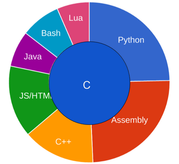
\includegraphics[scale=0.62]{img/test.png}
    ~
  \section{OS Knowledge}
    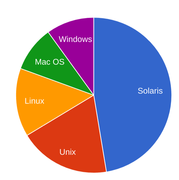
\includegraphics[scale=0.62]{img/os.png}
    ~
  \section{Tools/Utilities}
    \vspace{20pt}
    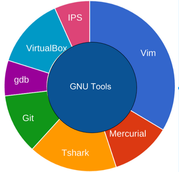
\includegraphics[scale=0.62]{img/tools.png}
    ~
\end{aside}

\section{Experience}
\begin{entrylist}
  \entry
    {09/15 - Now}
    {University of California, Santa Cruz}
    {Teaching Assistant/Grad. Student}
    {Teaching Assistant for undergrad course "Computer Systems and Assembly Language" for the Fall and Winter quarter}
    {}
  \entry
    {02/12 - 08/15}
    {Oracle India Pvt. Ltd.}
    {Software Engineer}
    {Worked for Oracle System's Group. Primarily fixed bugs in Solaris Kernel’s core networking components like TCP/IP, MAC, network level virtualization and utilities \\}
    {\textbf{Responsibilities and Competencies}
    \begin{itemize}
        \item Fixing bugs complex panics/crashes/hangs in both x86 and SPARC architectures.
        \item Security issues/projects and networking performance bugs.
        \item Debug tools like Dtrace, mdb and truss. 
        \item Sniffing tools like wireshark/tshark, snoop, tcpdump.
        \item Have worked on features for high availability like IPMP, aggregation, VRRP and virtualization technologies like LDoms, VNICs, zones, and flow control.
        \item Have given and attended TOIs/ unconferences to colleagues
        \item Have trained Solaris Network Administrators, Technical Writers and customers about new features.
        \item Code Integration processes such as Code Inspection/Reviews, Code Integration(RTI), Backporting and tools such as Mercurial, BugDB and grok.
        \item Worked extensively with other Unix-like environments, like bsd/linux and have compiled and ported multiple third party tools on them.
        \item Authored various cheat-sheets and articles for other teams to use.
        \item Maintaining servers in the local lab to create configurable/on demand virtual machines for team members to use - VirtualBox for x86 and Oracle VM for SPARC.
        \item Thorough understanding of Solaris kernel implementation.
        \item Conducted product promotion presentations for the Oracle Users Group community from various countries at Hyderabad.
        \item Received several appreciations/certifications/awards for solving highly complex issues.
    \end{itemize}
    }
\end{entrylist}

\begin{entrylist}
  \entry
    {10/10 - 01/12}
    {Huawei Technologies, Bangalore}
    {Software Engineer}
    {Worked at Huawei's research facility in Bangalore. For the most part researched, designed, prototyped and implemented several features of the SNMP protocol to support Huawei's OS (VRPV8) which is deployed on their routers and switches (NE5k series).}
    {\textbf{Responsibilities and Competencies}
    \begin{itemize}
        \item Developing a Common routing platform for most  Huawei Network and Communication equipment (Hands on experience with NE5k series of Routers).
        \item Developing features, fixing defects and resolving crashes.
        \item Actively involved in design phase brainstorming and writing SRS, HLD and LLD.
        \item Developed a feature to support SNMP Multi-VB Get-Bulk operation
        \item Added a feature to support private VB Traps/Informs
        \item Designed and coded a feature for an SNMP Agent to connect to a Manager based on FSM of Socket component in VRPV8.
        \item Worked on mcHuawei (Huawei's MIB Lex and YACC compiler) - Wrote a feature that converts RFC MIB files to a generic format which can be modified by L2/L3 protocols for their customized needs. 
    \end{itemize}
    }
\end{entrylist}

\begin{entrylist}
  \entry  
    {}{}{}{}
    {
    \begin{itemize}
        \item Worked extensively in development phase testing like UT, CT (CxxTest  framework) and IT. 
        \item Individually set up CT framework for SNMP. Also worked
          extensively in UT for improving code quality.
        \item Worked on IPC, Networking and DB.
        \item Software processes like Agile Software development life cycle.
          
    \end{itemize}
    }
\end{entrylist}

\section{Skills \& Strengths}
    \begin{itemize}
        \item Delivering bug free, maintainable and performance optimized             features/projects on-time.
        \item Very good at designing scalable and maintainable software. 
        \item In-depth knowledge of  OS concepts/C language.
        \item Can debug bugs/panics/hangs promptly and on short notice.
        \item Fast  learner, smart worker and excellent team player.
        \item Good at presentation and mentoring.
    \end{itemize}


\section{Education}
  \entry
    {2015 - 2016}
    {Masters of Computer Engg.}
    {Univ. of California, Santa Cruz}
    {Specialization in Networking. "Analysis of Algorithms"(A), "Computer Networks"(A-) }
    {}
  \entry
    {2005 - 2009}
    {Bachelors of Electronics and Communication Engg.}
    {Univ. of Calicut}
    {Graduated with First Class\\}
    {}    
\end{entrylist}

\section{Certifications and Contests}
    \begin{itemize}
        \item NIIT .Net Framework Certification
        \item Aptech Java Certification
        \item First prize for College Debugging in C Competition
        \item First prize for College Technical Quiz Competition
        \item Won multiple Math Skill Contests
        \item CBSE South Zone India Swimming Bronze Medalist
        \item Captained High School Basketball Team
    \end{itemize}

\vspace{40pt}
\begin{flushleft}
\emph{Priyesh Vakayil}
\end{flushleft}

%%% This piece of code has been commented by Karol Kozioł due to biblatex errors. 
% 
%\printbibsection{article}{article in peer-reviewed journal}
%\begin{refsection}
%  \nocite{*}
%  \printbibliography[sorting=chronological, type=inproceedings, title={international peer-reviewed conferences/proceedings}, notkeyword={france}, heading=subbibliography]
%\end{refsection}
%\begin{refsection}
%  \nocite{*}
%  \printbibliography[sorting=chronological, type=inproceedings, title={local peer-reviewed conferences/proceedings}, keyword={france}, heading=subbibliography]
%\end{refsection}
%\printbibsection{misc}{other publications}
%\printbibsection{report}{research reports}

\end{document}
